\documentclass[]{article}

% sottotitolo
\usepackage{titling}
\newcommand{\subtitle}[1]{%
  \posttitle{%
    \par\end{center}
    \begin{center}\large#1\end{center}
    \vskip0.5em}%
}

% accenti
\usepackage[utf8]{inputenc}
% rimuove indentatura
\usepackage[parfill]{parskip}
% colori
\usepackage{color}
% per cambiare i margini della pagina
\usepackage{vmargin}
% per fissare le figure
\usepackage{float}

\usepackage{graphicx}

% per formattare il codice Java
\usepackage{listings}
\definecolor{dkgreen}{rgb}{0,0.6,0}
\definecolor{gray}{rgb}{0.5,0.5,0.5}
\definecolor{mauve}{rgb}{0.58,0,0.82}
\lstset{frame=tb,
  language=Java,
  aboveskip=3mm,
  belowskip=3mm,
  showstringspaces=false,
  columns=flexible,
  basicstyle={\small\ttfamily},
  numbers=none,
  numberstyle=\tiny\color{gray},
  keywordstyle=\color{blue},
  commentstyle=\color{dkgreen},
  stringstyle=\color{mauve},
  breaklines=true,
  breakatwhitespace=true,
  tabsize=3
}

\begin{document}

\title{Autonoleggio}
\subtitle{Ingegneria del Software - Approfondimento}
\author{Federico Magnolfi}
\date{Gennaio 2018}
\maketitle

\section*{Introduzione}
In questo elaborato vengono approfonditi l'utilizzo di due pattern, Singleton e Observer, e l'utilizzo di buone pratiche da rispettare nella progettazione delle classi, per garantire il comportamento desiderato del programma.

Il Singleton è un pattern creazionale che ha lo scopo di assicurarsi che una classe abbia una sola istanza e provvedere un punto di accesso globale a questa istanza.

L'Observer è un pattern comportamentale che permette di definire una dipendenza uno a molti tra oggetti in modo che quando un oggetto cambia stato, vengano notificati tutti i i suoi osservatori.

\section*{Scenario}
Per descrivere quanto detto nell'introduzione, si è scelto di rappresentare lo scenario di un autonoleggio. L'autonoleggio dispone di un certo numero di macchine. Un utente può chiedere all'autonoleggio l'affitto di una macchina. Se ce n'è una disponibile, viene assegnata all'utente che la può usare quanto vuole, fino a quando non decide di riportarla all'autonoleggio. Se invece non ci sono macchine disponibili all'affitto, l'utente viene aggiunto alla lista di persone che verranno notificate quando ci saranno delle macchine libere. Si vuole inoltre che ogni utente al massimo possa affittare una macchina alla volta.

\section*{Analisi e progettazione}
Nel sistema saranno presenti quattro classi principali: una per l'autonoleggio (CarRental), una per le macchine (Car), una per gli utenti(User), e una per testare il funzionamento (Test).

L'autonoleggio in questione è uno soltanto, per imporre questo vincolo si usa il pattern del Singleton applicato alla classe CarRental.
Per permettere all'autonoleggio di inviare notifiche agli utenti riguardo alla disponibilità delle auto, si usa il pattern dell'Observer: CarRental è il subject concreto, mentre User è l'observer concreto, si sfruttano la classe Observable e l'interfaccia Observer predefinite di Java.

Per il corretto funzionamento di tutto il sistema, è necessaria una stretta collaborazione tra le varie classi, ognuna delle quali ha delle responsabilità a cui non si può sottrarre.
Si è data particolare importanza ai modificatori di visibilità, per garantire che nessuna classe possa eseguire operazioni che non le sono permesse.
Per evitare utilizzi diversi a questa progettazione, si è deciso di rendere final ogni classe, ovvero non estendibile.


\section*{Partecipanti}
\begin{itemize}
\item \textbf{Car}: la classe Car è una classe statica interna a CarRental, questo serve per permettere all'autonoleggio di accedere direttamente ai campi privati delle macchine, ed allo stesso tempo impedire la modifica di questi ad altre classi, anche dello stesso package; in particolare la classe Car ha il costruttore privato, quindi solo l'autonoleggio può instanziare nuove macchine, lo stesso meccanismo è usato per il metodo \textit{setRenter(User)}, che permette l'impostazione dell'affittuario dell'auto.
\item \textbf{CarRental}: la classe CarRental mette a disposizione un metodo package-private \textit{rentCar(User)} per permettere agli utenti di richiedere una macchina da affittare: si è scelto di non dare la macchina come valore di ritorno, che potrebbe anche essere "perso", si è quindi deciso di invertire la responsabilità di impostare la macchina affittata dall'utente, affidando questa al CarRental, è quindi necessario un parametro per sapere chi è l'utente che vuole affittare la macchina; conoscere chi vuole affittare una macchina serve anche per assicurarsi che ogni persona non possa affittare più di una macchina alla volta. È inoltre presente un metodo \textit{returnCar(User)} che permette di restituire la macchina.

\item \textbf{User}: la classe User, ha quattro metodi pubblici che consentono di ottenere il nome dell'utente (\textit{getName()}), affittare (\textit{rentCar()}), utilizzare (\textit{useCar()}) e rendere (\textit{returnCar()}) la macchina; possiede anche due metodi package-private che servono per impostare (\textit{setCar(Car)}) e ottenere (\textit{getCar()}) la macchina noleggiata: in questo modo si è sicuri che soltanto l'autonoleggio può cambiare e vedere la macchina che è stata assegnata.
\item \textbf{Test}: testa il funzionamento del sistema.
\end{itemize}

\clearpage
\section*{Class Diagram}
Si riporta di seguito il Class Diagram UML del sistema (Figura \ref{imgClassDiagram}).

\begin{figure}[H]
	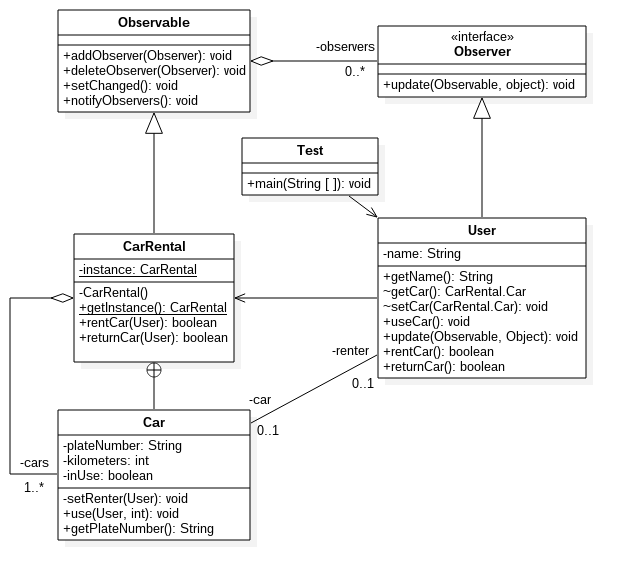
\includegraphics[width=\linewidth]{img/Rental_UML_ClassDiagram.jpg}
	\caption{Class Diagram}
	\label{imgClassDiagram}
\end{figure}

\clearpage
\section*{Sequence Diagram}
Si riporta di seguito il Sequence Diagram UML (Figura \ref{imgSequenceDiagram}) relativo a quando dal test si crea un utente, si comanda poi all'utente di affittare una macchina.

\begin{figure}[H]
	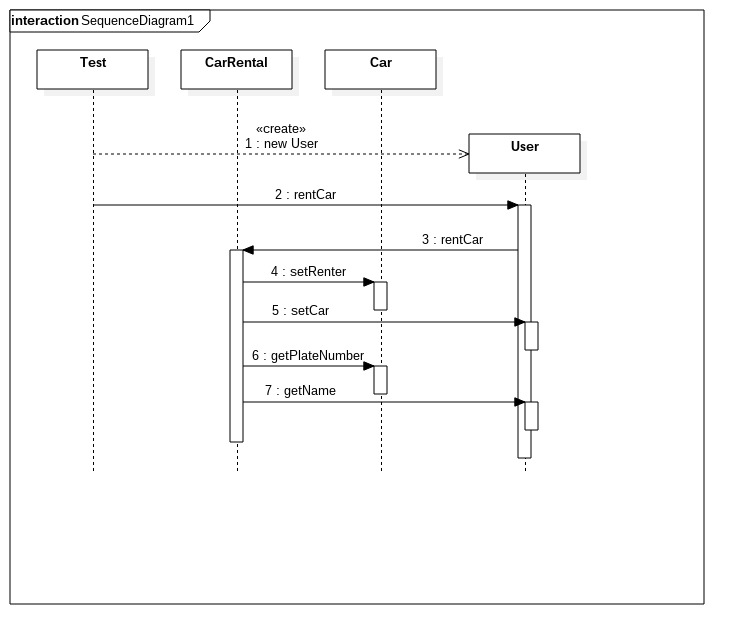
\includegraphics[width=\linewidth]{img/Rental_UML_SequenceDiagram.jpg}
	\caption{Sequence Diagram}
	\label{imgSequenceDiagram}
\end{figure}

\clearpage
\section*{Codice}
Si riporta di seguito il codice del programma Java, suddiviso per file.

\subsubsection*{CarRental.java}
\begin{lstlisting}
package com.federicomagnolfi;
import java.util.ArrayList;
import java.util.Observable;

public final class CarRental extends Observable
{
    public static final class Car
    {
        private final String plateNumber;   // plate number of the car
        private int kilometers;             // kilometers done by the car
        private boolean inUse;              // true if someone has rented this car
        private User renter;                // user that rented this car

        private Car(String plateNumber)
        {   // constructor is private, only the CarRental can instantiate a Car
            this.plateNumber = plateNumber;
            kilometers = 0;
            inUse = false;
        }

        // private method, only the CarRental can change the renter of the car
        private void setRenter(User renter)
        {
            this.renter = renter;
        }

        public void use(User user, int kilometers)
        {
            // check appropriate use of the car
            if(user != renter)
                throw new Error("Only the renter can use the car!");
            // increment kilometers counter
            this.kilometers += kilometers;

            System.out.println("Car " + getPlateNumber() + " used for " + kilometers + " km by user " + user.getName() + ". Total km of the car: " + this.kilometers);
        }

        public String getPlateNumber()
        {
            // returns the plate number, yellow colored
            return "\033[32m" + plateNumber + "\033[0m";
        }
    }


    private static CarRental instance;          // only instance of the CarRental

    private final ArrayList<Car> cars;          // list of cars owned by the CarRental

    private CarRental()
    {
        final int carsNumber = 2;               // total cars owned by the CarRental
        cars = new ArrayList<>();
        for (int i = 0; i < carsNumber; i++)
        {
            cars.add(new Car("IT" + (101+i + "FM")));
        }
    }

    public static CarRental getInstance()
    {   // returns the unique instance
        if(instance == null)
            instance = new CarRental();
        return instance;
    }

    // returns true if car is rented, false otherwise
    boolean rentCar(User renter)
    {
        for(Car car: cars)
        {
            if(car.renter == renter)
            {
                System.out.println("Every user can rent one car at most");
                return false;
            }
        }
        for(Car car: cars)
        {   // search for an available car
            if(!car.inUse)
            {   // if an available car is found, it's assigned to the user
                car.inUse = true;
                car.setRenter(renter);
                renter.setCar(car);
                System.out.println("Car " + car.getPlateNumber() + " assigned to " + renter.getName());
                return true;
            }
        }
        // if no car is available
        addObserver(renter);
        System.out.println("User " + renter.getName() + " will be notified as soon as a car returns available");
        return false;
    }

    // returns true if the car is effectively returned, false otherwise
    boolean returnCar(User user)
    {
        Car car = user.getCar();
        if (cars.indexOf(car) != -1)
        {   // car is prepared to be rented again
            car.inUse = false;
            car.setRenter(null);
            user.setCar(null);  // user lose the reference to use the car
            System.out.println("User " + user.getName() + " has returned the car " + car.getPlateNumber());
            setChanged();
            notifyObservers();
            return true;
        }
        System.out.println("The user did not rent a car, so he can't return a car");
        return false;
    }
}

\end{lstlisting}

\subsubsection*{User.java}
\begin{lstlisting}
package com.federicomagnolfi;
import java.util.Observable;
import java.util.Observer;

public final class User implements Observer
{
    private final String name;
    private CarRental.Car car;

    public User(String name)
    {
        this.name = name;
    }

    public String getName()
    {
        // returns the name, blue colored
        return "\033[34m" + name + "\033[0m";
    }

    CarRental.Car getCar()
    {
        return car;
    }

    void setCar(CarRental.Car car)
    {
        this.car = car;
    }

    public void useCar()
    {
        // check if this user does have a car
        if(car != null)
            // if he has a car, he use it
            car.use(this, (int) (1 + Math.random()*20));
        else
            System.out.println("User " + getName() + " doesn't have a car to use");
    }

    @Override
    public void update(Observable observable, Object o)
    {   // receives the notification that a car is available
        System.out.println("User " + getName() + " receives the notification");
        CarRental.getInstance().deleteObserver(this);    // unsubscribes from list
        // now he can ask to rent a car again...
    }

    public boolean rentCar()
    {
        return CarRental.getInstance().rentCar(this);
    }

    public boolean returnCar()
    {
        return CarRental.getInstance().returnCar(this);
    }
}

\end{lstlisting}

\subsubsection*{Test.java}
\begin{lstlisting}
package com.federicomagnolfi;

public class Test
{
    public static void main(String[] args)
    {

        User user1 = new User("FedeMagno");
        User user2 = new User("GiuliF");
        User user3 = new User("Stefano");
        User user4 = new User("Andrea");

        user1.rentCar();
        user2.rentCar();
        user3.rentCar();
        user4.rentCar();

        user1.useCar();
        user2.useCar();
        user3.useCar();
        user4.useCar();

        user1.returnCar();
        user2.returnCar();
        user3.returnCar();
        user4.returnCar();

    }
}

\end{lstlisting}

\subsubsection*{Output}
\begin{verbatim}
Car IT101FM assigned to FedeMagno
Car IT102FM assigned to GiuliF
User Stefano will be notified as soon as a car returns available
User Andrea will be notified as soon as a car returns available
Car IT101FM used for 15 km by user FedeMagno. Total km of the car: 15
Car IT102FM used for 5 km by user GiuliF. Total km of the car: 5
User Stefano doesn't have a car to use
User Andrea doesn't have a car to use
User FedeMagno has returned the car IT101FM
User Andrea receives the notification
User Stefano receives the notification
User GiuliF has returned the car IT102FM
The user did not rent a car, so he can't return a car
The user did not rent a car, so he can't return a car
\end{verbatim}

   
\end{document}